
%
%%----------------------------------------------------------------


\section{Modelo de información: Módulo Oferta Educativa}
\subsection{Módulo Plan de Estudio: Descripción general}
En la figura~\ref{fig:planEstudio} se muestra la estructura de información que manejará el módulo Plan de estudio.

\begin{figure}[htbp!]
	\begin{center}
		\fbox{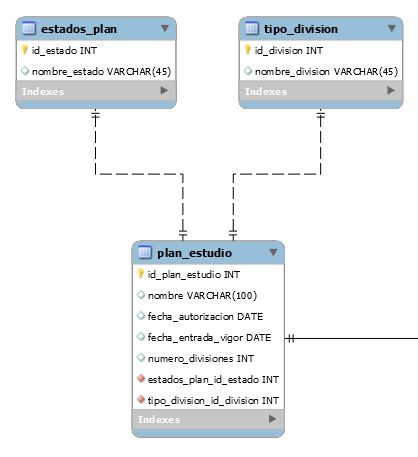
\includegraphics[width=.5\textwidth]{images/clases/PlanEstudio.png}}
		\caption{Modelo de información del módulo Plan de estudio.}
		\label{fig:planEstudio}
	\end{center}
\end{figure}

%--------------------------------------------------------------------------------
\begin{BusinessEntity}{planEstudio}{Plan de estudio}
	
	\Battr{nombre}{Nombre}{\tdFrase}{Es el nombre con el que se registra el edificio}{\requerido}{\longitudMax{50}{caracteres}}{Caracteres admitidos: [A-Z] $|$ [a-z] $|$ [1-9] $|$ \_ $|$ $-$ $|$ [á,é,é,ó,ú]  $|$ [Á,É,Í,Ó,Ú] $|$ \textvisiblespace.}
	
	\Battr{fechaAutorizacion}{Fecha de autorización}{\tdFecha}{Es el día en el que el plan de estudio fue autorizado}{\requerido}

	\Battr{fechaEntradaVigor}{Fecha de entrega en vigor}{\tdFecha}{Es el día en el que el plan de estudio entra en vigor}{\requerido}
	
	\Battr{numeroDivisiones}{Divisiones}{\tdNumerico}{De acuerdo al tipo de división, indica cuantas divisiones tiene el plan de estudio.}{\requerido}{\longitudMinMax{1}{caracteres}{2}{caracteres}}{Caracteres admitidos: [0-9].}
	
\end{BusinessEntity}


%--------------------------------------------------------------------------------
\begin{BusinessEntity}{tipoDivision}{Tipo de division}
	
	\Battr{nombreDivision}{División}{\tdCatalogo}{Es el tipo de division que tiene el plan de estudio, como son: \begin{itemize}
			\item Semestres 
			\item Nivel 
		\end{itemize}
	}{\requerido}
\end{BusinessEntity}
%--------------------------------------------------------------------------------

\subsection{Módulo Unidad de Aprendizaje: Descripción general}
En la figura~\ref{fig:unidadAprendizaje} se muestra la estructura de información que manejará el módulo Unidad de Aprendizaje.

\begin{figure}[htbp!]
	\begin{center}
		\fbox{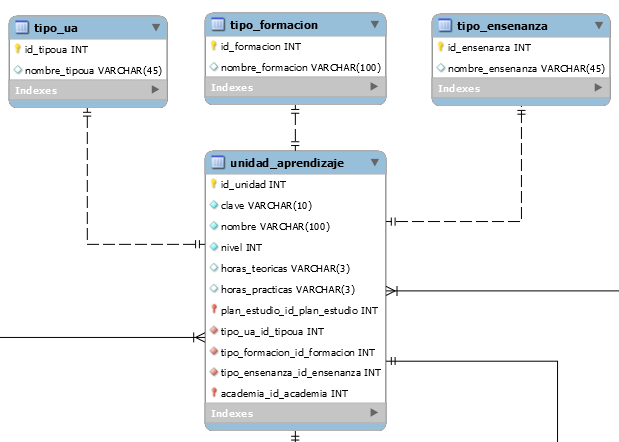
\includegraphics[width=.5\textwidth]{images/clases/UnidadAprendizaje.png}}
		\caption{Modelo de información del módulo Unidad de Aprendizaje.}
		\label{fig:unidadAprendizaje}
	\end{center}
\end{figure}

%--------------------------------------------------------------------------------
\begin{BusinessEntity}{unidadAprendizaje}{Unidad de aprendizaje}

	\Battr{clave}{Clave}{\tdPalabra}{Es la clave asignada a la unidad de aprendizaje como única}{\requerido}{\longitudMax{10}{caracteres}}{Caracteres admitidos: [A-Z] $|$ [a-z] $|$ [1-9].}
	
	\Battr{nombre}{Nombre}{\tdFrase}{Es el nombre con el que se registra la unidad de aprendizaje}{\requerido}{\longitudMax{100}{caracteres}}{Caracteres admitidos: [A-Z] $|$ [a-z] $|$ [1-9] $|$ $-$ $|$ [á,é,é,ó,ú]  $|$ [Á,É,Í,Ó,Ú] $|$ \textvisiblespace.}
	
	\Battr{nivel}{Nivel}{\tdNumerico}{Es el número del nivel al que pertenece la unidad de aprendizaje}{\requerido}{\longitudMinMax{1}{caracteres}{2}{caracteres}}{Caracteres admitidos: [0-9].}
	
	\Battr{horasTeoricas}{Horas teóricas}{\tdPalabra}{Es el número de horas teóricas de la unidad de aprendizaje}{\requerido}{\longitudMax{3}{caracteres}}{Caracteres admitidos: [1-9] $|$ $.$.}
	
	\Battr{horasPracticas}{Horas prácticas}{\tdPalabra}{Es el número de horas prácticas de la unidad de aprendizaje}{\requerido}{\longitudMax{3}{caracteres}}{Caracteres admitidos: [1-9] $|$ $.$.}
		
\end{BusinessEntity}

%--------------------------------------------------------------------------------
\begin{BusinessEntity}{tipoUA}{Tipo de unidad de aprendizaje}
	
		\Battr{nombreTipoUA}{Tipo de ua}{\tdCatalogo}{Indica el tipo de unidad de aprendizaje, los posibles tipos son: \begin{itemize}
			\item Obligatoria 
			\item Optativa
		\end{itemize}
	}{\requerido}
	
\end{BusinessEntity}

%--------------------------------------------------------------------------------
\begin{BusinessEntity}{tipoFormacion}{Tipo de formación}
	
	\Battr{nombre}{Tipo de espacio}{\tdCatalogo}{Es el tipo de formación que tiene la unidad de aprendizaje, como son: \begin{itemize}
			\item Formación Institucional
			\item Formación Científica-Básica
			\item Formación Profesional 
			\item Formación Terminal e Integral 
		\end{itemize}
	}{\requerido}
	
\end{BusinessEntity}


%--------------------------------------------------------------------------------
\begin{BusinessEntity}{tipoEnsenanza}{Tipo de enseñanza}
	
	\Battr{nombre}{Tipo de ensenanza}{\tdCatalogo}{Es el tipo de enseñanza que tiene la unidad de aprendizaje, como son: \begin{itemize}
			\item Teórico
			\item Práctica
			\item Teórica-Prácticas
		\end{itemize}
	}{\requerido}
	
\end{BusinessEntity}


%--------------------------------------------------------------------------------